\documentclass[12pt, twoside]{article}
% \documentclass[12pt, twoside]{article}
\usepackage[letterpaper, margin=1in, headsep=0.2in]{geometry}
\setlength{\headheight}{0.6in}
%\usepackage[english]{babel}
\usepackage[utf8]{inputenc}
\usepackage{microtype}
\usepackage{amsmath}
\usepackage{amssymb}
%\usepackage{amsfonts}
\usepackage[nomessages]{fp} %\FPeval{\var-name}{2*sin(pi/6)}
\usepackage{siunitx} %units in math. eg 20\milli\meter
\usepackage{yhmath} % for arcs, overparenth command
\usepackage{tikz} %graphics
\usetikzlibrary{quotes, angles, arrows, arrows.meta}
\usepackage{graphicx} %consider setting \graphicspath{{images/}}
\usepackage{parskip} %no paragraph indent
\usepackage{enumitem}
\usepackage{multicol}
\usepackage{venndiagram}

\usepackage{fancyhdr}
\pagestyle{fancy}
\fancyhf{}
\renewcommand{\headrulewidth}{0pt} % disable the underline of the header
\raggedbottom
\hfuzz=2mm %suppresses overfull box warnings

\usepackage{hyperref}
\usepackage{float}

\title{Algebra 2}
\author{Chris Huson}
\date{June 2024}

\fancyhead[LE]{\thepage}
\fancyhead[RO]{\thepage \\ Name: \hspace{1.5cm} \,\\}
\fancyhead[LO]{BECA/Huson/Algebra 2: Regents Preparation \\* 7 June 2024}

\begin{document}
\subsubsection*{Prep \#25 Periodic functions}
\begin{enumerate}
\item Graph the function $f(x)= 2 \sin x +6$. Notate the midline, amplitude, relative minimum and maximum, zeros.
    \begin{center}
    \begin{tikzpicture}[xscale=2, yscale=0.8]
        \draw[gray,thin] (0,0) grid[xstep=pi/8] (6.3,9);
        \draw [thick,->] (0,0)--(6.5,0) node [right] {$x$};
        \draw [thick,->] (0,0)--(0,9.5) node [right] {$y$};
        \foreach \x/\xtext in {0.5*pi/$\frac{1}{2}\pi$, pi/$\pi$, 1.5*pi/$\frac{3}{2}\pi$,2*pi/$2\pi$}
            \draw (\x,5pt) -- (\x,-5pt) node[below] {\xtext};
        \foreach \y in {0,...,9}
            \draw (2pt,\y cm)--(-2pt,\y cm) node[left]{$\y$};
    \end{tikzpicture}
    \end{center}
        
\item The function $f(x)= \sin x$ is shown on the graph below as well as two other periodic functions, $g(x)$ and $h(x)$. Write down the period and equation for each function.
    \begin{center}
    \begin{tikzpicture}[xscale=2]
        \draw[gray,thin] (0,-4) grid[xstep=pi/8] (6.3,3);
        \draw [thick,->] (0,0)--(6.5,0) node [below right] {$x$};
        \draw [thick,->] (0,-4)--(0,3.5) node [right] {$y$};
        \foreach \x/\xtext in {0.5*pi/$\frac{1}{2}\pi$, pi/$\pi$, 1.5*pi/$\frac{3}{2}\pi$,2*pi/$2\pi$}
            \draw (\x,5pt) -- (\x,-5pt) node[below] {\xtext};
        \foreach \y in {-4,...,3}
            \draw (2pt,\y cm)--(-2pt,\y cm) node[left]{$\y$};
        \draw [thick,->, domain=0:2*pi+0.25,smooth,samples=100] plot (\x,{sin(\x r)}) node [above right]{$f(x)$};
        \draw [thick,->, domain=0:2*pi+0.1,smooth,samples=100] plot (\x,{2+sin(2*\x r)}) node [above right]{$g(x)$};
        \draw [thick,->, domain=0:2*pi+0.1,smooth,samples=100] plot (\x,{-3+sin(pi *\x r)}) node [below right]{$h(x)$};
        \fill (pi,2) ellipse (1pt and 2pt);
        \fill (2,-3) ellipse (1pt and 2pt);
        \draw [thick,<->] (0,-2.6) -- (2,-2.6);
        \draw [thick,dashed] (2,-3) -- (2,0) node [above] {2};
    \end{tikzpicture}
    \end{center}


\newpage
\item A person's lung capacity can be modeled by the function $\displaystyle C(t) = 250\sin(\frac{2\pi}{5} t) = 2450$, where $C(t)$ represents the volume in mL present in the lungs after $t$ seconds. State the maximum value of this function over one full cycle, and explain what this value represents. %Regents Aug2019
\vspace{5cm}

\item A periodic function $f(x)$ is shown on the graph below.
\begin{enumerate}
    \item Write down the amplitude, period, and midline equation of the function. \vspace{2cm}
    \begin{center}
        \begin{tikzpicture}[xscale=1, yscale=0.4]
            \draw[gray,thin] (0,0) grid[xstep=1,ystep=2] (10.3,18);
            \draw [thick,->] (0,0)--(10.5,0) node [right] {$x$};
            \draw [thick,->] (0,0)--(0,18.5) node [above] {$f(x)$};
            \foreach \x in {1,...,10}
                \draw (\x,5pt) -- (\x,-5pt) node[below] {$\x$};
            \foreach \y in {0,2,...,18}
                \draw (2pt,\y cm)--(-2pt,\y cm) node[left]{$\y$};
            \draw [thick,->, domain=0:10.2,smooth,samples=100] plot (\x,{3*sin(\x *pi/3 r)+12});
            \fill (1.5,15) ellipse (2pt and 5pt);
            \fill (3,12) ellipse (2pt and 5pt);
            \fill (4.5,9) ellipse (2pt and 5pt);
            \fill (6,12) ellipse (2pt and 5pt);
            \end{tikzpicture}
        \end{center}
        \item Write the equation for $f(x)$.
    \end{enumerate}

\newpage
\item Write a recursive formula for the sequence 121, 12.1, 1.21, 0.121, $\ldots$ \vspace{3cm}

\item When a ball bounces, the heights of consecutive bounces form a geometric sequence. The height of the first bounce is 121 centimeters and the height of the third bounce is 64 centimeters. To the \emph{nearest centimeter}, what is the height of the fifth bounce? %Regents Jan2019
    \begin{center}
    \begin{tabular}{|p{3cm}|p{1cm}|p{1cm}|p{1cm}|p{1cm}|p{1cm}|}
        \hline
        bounce & 1 & 2 & 3 & 4 & 5 \\
        \hline
        height (cm) & 121 & & 64 & & \\[0.25cm]
        \hline
    \end{tabular}
    \end{center}
\vspace{5cm}

\item Rowan is training to run in a race. He runs 15 miles in the first week, and each week following, he runs 3\% more than the week before. Using a geometric series formula, find the total number of miles Rowan runs over the first ten weeks of training, rounded to the \emph{nearest thousandth}. %Regents Jan2019

\newpage
\item Given $P(A) = \frac{1}{3}$ and $P(B) = \frac{5}{12}$, where $A$ and $B$ are independent events. Determine $P(A \cap B)$. \vspace{3cm}

\item The set of data in the table below shows the results of a survey on the number of messages that people of different ages text on their cell phones each month.
\begin{center}
    \begin{tabular}{|c|c|c|c|}
        \hline
        Age Group & 0-10 & 11-50 & Over 50 \\
        \hline
        15-18 & 4 & 37 & 68 \\[0.25cm]
        \hline
        19-22 & 6 & 25 & 87 \\[0.25cm]
        \hline
        23-60 & 25 & 47 & 157 \\[0.25cm]
        \hline
    \end{tabular}
\end{center}
If a person from this survey is selected at random, what is the probability that the person texts over 50 messages per month given that the person is between the ages of 23 and 60?  \vspace{4cm}

\item The scores on a collegiate mathematics readiness assessment are approximately normally distributed with a mean of 680 and a standard deviation of 120.\\[0.5cm]
Determine the percentage of scores between 690 and 900, to the \emph{nearest percent}.\vspace{3cm}




\end{enumerate}
\end{document}